\documentclass[border=4pt]{standalone}

\usepackage{amsmath}
\usepackage{tikz}
\usepackage{mathdots}
\usepackage{yhmath}
\usepackage{cancel}
\usepackage{color}
\usepackage{siunitx}
\usepackage{array}
\usepackage{multirow}
\usepackage{amssymb}
\usepackage{gensymb}
\usepackage{tabularx}
\usepackage{booktabs}
\usetikzlibrary{fadings}
\usetikzlibrary{patterns}


\begin{document}
 
\tikzset{every picture/.style={line width=0.75pt}} %set default line width to 0.75pt

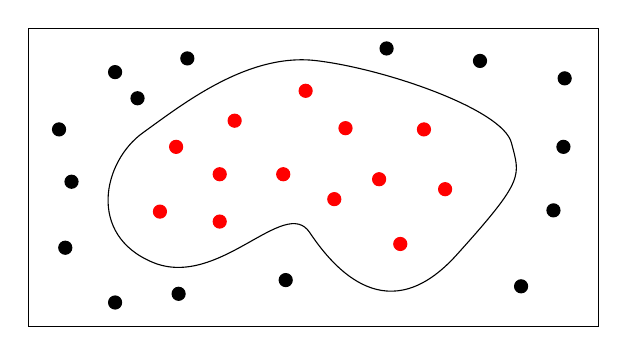
\begin{tikzpicture}[x=0.75pt,y=0.75pt,yscale=-0.6,xscale=0.6]
%uncomment if require: \path (0,300); %set diagram left start at 0, and has height of 300

%Shape: Rectangle [id:dp19586351230379806]
\draw   (80,20) -- (538,20) -- (538,259.48) -- (80,259.48) -- cycle ;
%Shape: Polygon Curved [id:ds7033458632402881]
\draw   (172,104) .. controls (204,81) and (256.25,39.63) .. (311,46) .. controls (365.75,52.37) and (461,85) .. (468,112) .. controls (475,139) and (479,141) .. (424,202) .. controls (369,263) and (326,214) .. (306,184) .. controls (286,154) and (233,230) .. (180,208) .. controls (127,186) and (140,127) .. (172,104) -- cycle ;
%Shape: Circle [id:dp6951665056576987]
\draw  [fill={rgb, 255:red, 0; green, 0; blue, 0 }  ,fill opacity=1 ] (144.51,55.24) .. controls (144.51,52.35) and (146.86,50) .. (149.76,50) .. controls (152.65,50) and (155,52.35) .. (155,55.24) .. controls (155,58.14) and (152.65,60.49) .. (149.76,60.49) .. controls (146.86,60.49) and (144.51,58.14) .. (144.51,55.24) -- cycle ;
%Shape: Circle [id:dp09237665476213075]
\draw  [fill={rgb, 255:red, 0; green, 0; blue, 0 }  ,fill opacity=1 ] (144.51,240.24) .. controls (144.51,237.35) and (146.86,235) .. (149.76,235) .. controls (152.65,235) and (155,237.35) .. (155,240.24) .. controls (155,243.14) and (152.65,245.49) .. (149.76,245.49) .. controls (146.86,245.49) and (144.51,243.14) .. (144.51,240.24) -- cycle ;
%Shape: Circle [id:dp9815932756793359]
\draw  [fill={rgb, 255:red, 0; green, 0; blue, 0 }  ,fill opacity=1 ] (99.51,101.24) .. controls (99.51,98.35) and (101.86,96) .. (104.76,96) .. controls (107.65,96) and (110,98.35) .. (110,101.24) .. controls (110,104.14) and (107.65,106.49) .. (104.76,106.49) .. controls (101.86,106.49) and (99.51,104.14) .. (99.51,101.24) -- cycle ;
%Shape: Circle [id:dp4306114970629712]
\draw  [fill={rgb, 255:red, 0; green, 0; blue, 0 }  ,fill opacity=1 ] (104.51,196.24) .. controls (104.51,193.35) and (106.86,191) .. (109.76,191) .. controls (112.65,191) and (115,193.35) .. (115,196.24) .. controls (115,199.14) and (112.65,201.49) .. (109.76,201.49) .. controls (106.86,201.49) and (104.51,199.14) .. (104.51,196.24) -- cycle ;
%Shape: Circle [id:dp2460866722278987]
\draw  [fill={rgb, 255:red, 0; green, 0; blue, 0 }  ,fill opacity=1 ] (470.51,227.24) .. controls (470.51,224.35) and (472.86,222) .. (475.76,222) .. controls (478.65,222) and (481,224.35) .. (481,227.24) .. controls (481,230.14) and (478.65,232.49) .. (475.76,232.49) .. controls (472.86,232.49) and (470.51,230.14) .. (470.51,227.24) -- cycle ;
%Shape: Circle [id:dp5988893118600079]
\draw  [fill={rgb, 255:red, 0; green, 0; blue, 0 }  ,fill opacity=1 ] (437.51,46.24) .. controls (437.51,43.35) and (439.86,41) .. (442.76,41) .. controls (445.65,41) and (448,43.35) .. (448,46.24) .. controls (448,49.14) and (445.65,51.49) .. (442.76,51.49) .. controls (439.86,51.49) and (437.51,49.14) .. (437.51,46.24) -- cycle ;
%Shape: Circle [id:dp7955065754248104]
\draw  [fill={rgb, 255:red, 0; green, 0; blue, 0 }  ,fill opacity=1 ] (202.51,44.24) .. controls (202.51,41.35) and (204.86,39) .. (207.76,39) .. controls (210.65,39) and (213,41.35) .. (213,44.24) .. controls (213,47.14) and (210.65,49.49) .. (207.76,49.49) .. controls (204.86,49.49) and (202.51,47.14) .. (202.51,44.24) -- cycle ;
%Shape: Circle [id:dp5320368700231608]
\draw  [fill={rgb, 255:red, 0; green, 0; blue, 0 }  ,fill opacity=1 ] (195.51,233.24) .. controls (195.51,230.35) and (197.86,228) .. (200.76,228) .. controls (203.65,228) and (206,230.35) .. (206,233.24) .. controls (206,236.14) and (203.65,238.49) .. (200.76,238.49) .. controls (197.86,238.49) and (195.51,236.14) .. (195.51,233.24) -- cycle ;
%Shape: Circle [id:dp8626471670475084]
\draw  [fill={rgb, 255:red, 0; green, 0; blue, 0 }  ,fill opacity=1 ] (162.51,76.24) .. controls (162.51,73.35) and (164.86,71) .. (167.76,71) .. controls (170.65,71) and (173,73.35) .. (173,76.24) .. controls (173,79.14) and (170.65,81.49) .. (167.76,81.49) .. controls (164.86,81.49) and (162.51,79.14) .. (162.51,76.24) -- cycle ;
%Shape: Circle [id:dp6749591223713287]
\draw  [fill={rgb, 255:red, 0; green, 0; blue, 0 }  ,fill opacity=1 ] (109.51,143.24) .. controls (109.51,140.35) and (111.86,138) .. (114.76,138) .. controls (117.65,138) and (120,140.35) .. (120,143.24) .. controls (120,146.14) and (117.65,148.49) .. (114.76,148.49) .. controls (111.86,148.49) and (109.51,146.14) .. (109.51,143.24) -- cycle ;
%Shape: Circle [id:dp8405392694619106]
\draw  [fill={rgb, 255:red, 0; green, 0; blue, 0 }  ,fill opacity=1 ] (496.51,166.24) .. controls (496.51,163.35) and (498.86,161) .. (501.76,161) .. controls (504.65,161) and (507,163.35) .. (507,166.24) .. controls (507,169.14) and (504.65,171.49) .. (501.76,171.49) .. controls (498.86,171.49) and (496.51,169.14) .. (496.51,166.24) -- cycle ;
%Shape: Circle [id:dp48499325988120323]
\draw  [fill={rgb, 255:red, 0; green, 0; blue, 0 }  ,fill opacity=1 ] (504.51,115.24) .. controls (504.51,112.35) and (506.86,110) .. (509.76,110) .. controls (512.65,110) and (515,112.35) .. (515,115.24) .. controls (515,118.14) and (512.65,120.49) .. (509.76,120.49) .. controls (506.86,120.49) and (504.51,118.14) .. (504.51,115.24) -- cycle ;
%Shape: Circle [id:dp8719681773533126]
\draw  [fill={rgb, 255:red, 0; green, 0; blue, 0 }  ,fill opacity=1 ] (505.51,60.24) .. controls (505.51,57.35) and (507.86,55) .. (510.76,55) .. controls (513.65,55) and (516,57.35) .. (516,60.24) .. controls (516,63.14) and (513.65,65.49) .. (510.76,65.49) .. controls (507.86,65.49) and (505.51,63.14) .. (505.51,60.24) -- cycle ;
%Shape: Circle [id:dp11963221191379259]
\draw  [fill={rgb, 255:red, 0; green, 0; blue, 0 }  ,fill opacity=1 ] (362.51,36.24) .. controls (362.51,33.35) and (364.86,31) .. (367.76,31) .. controls (370.65,31) and (373,33.35) .. (373,36.24) .. controls (373,39.14) and (370.65,41.49) .. (367.76,41.49) .. controls (364.86,41.49) and (362.51,39.14) .. (362.51,36.24) -- cycle ;
%Shape: Circle [id:dp570138793315528]
\draw  [fill={rgb, 255:red, 0; green, 0; blue, 0 }  ,fill opacity=1 ] (281.51,222.24) .. controls (281.51,219.35) and (283.86,217) .. (286.76,217) .. controls (289.65,217) and (292,219.35) .. (292,222.24) .. controls (292,225.14) and (289.65,227.49) .. (286.76,227.49) .. controls (283.86,227.49) and (281.51,225.14) .. (281.51,222.24) -- cycle ;
%Shape: Circle [id:dp24035863807399427]
\draw  [color={rgb, 255:red, 255; green, 0; blue, 0 }  ,draw opacity=1 ][fill={rgb, 255:red, 255; green, 0; blue, 0 }  ,fill opacity=1 ] (193.51,115.24) .. controls (193.51,112.35) and (195.86,110) .. (198.76,110) .. controls (201.65,110) and (204,112.35) .. (204,115.24) .. controls (204,118.14) and (201.65,120.49) .. (198.76,120.49) .. controls (195.86,120.49) and (193.51,118.14) .. (193.51,115.24) -- cycle ;
%Shape: Circle [id:dp7619219144290053]
\draw  [color={rgb, 255:red, 255; green, 0; blue, 0 }  ,draw opacity=1 ][fill={rgb, 255:red, 255; green, 0; blue, 0 }  ,fill opacity=1 ] (228.51,137.24) .. controls (228.51,134.35) and (230.86,132) .. (233.76,132) .. controls (236.65,132) and (239,134.35) .. (239,137.24) .. controls (239,140.14) and (236.65,142.49) .. (233.76,142.49) .. controls (230.86,142.49) and (228.51,140.14) .. (228.51,137.24) -- cycle ;
%Shape: Circle [id:dp7874306930139311]
\draw  [color={rgb, 255:red, 255; green, 0; blue, 0 }  ,draw opacity=1 ][fill={rgb, 255:red, 255; green, 0; blue, 0 }  ,fill opacity=1 ] (279.51,137.24) .. controls (279.51,134.35) and (281.86,132) .. (284.76,132) .. controls (287.65,132) and (290,134.35) .. (290,137.24) .. controls (290,140.14) and (287.65,142.49) .. (284.76,142.49) .. controls (281.86,142.49) and (279.51,140.14) .. (279.51,137.24) -- cycle ;
%Shape: Circle [id:dp5183165977477909]
\draw  [color={rgb, 255:red, 255; green, 0; blue, 0 }  ,draw opacity=1 ][fill={rgb, 255:red, 255; green, 0; blue, 0 }  ,fill opacity=1 ] (297.51,70.24) .. controls (297.51,67.35) and (299.86,65) .. (302.76,65) .. controls (305.65,65) and (308,67.35) .. (308,70.24) .. controls (308,73.14) and (305.65,75.49) .. (302.76,75.49) .. controls (299.86,75.49) and (297.51,73.14) .. (297.51,70.24) -- cycle ;
%Shape: Circle [id:dp04931338047052314]
\draw  [color={rgb, 255:red, 255; green, 0; blue, 0 }  ,draw opacity=1 ][fill={rgb, 255:red, 255; green, 0; blue, 0 }  ,fill opacity=1 ] (228.51,175.24) .. controls (228.51,172.35) and (230.86,170) .. (233.76,170) .. controls (236.65,170) and (239,172.35) .. (239,175.24) .. controls (239,178.14) and (236.65,180.49) .. (233.76,180.49) .. controls (230.86,180.49) and (228.51,178.14) .. (228.51,175.24) -- cycle ;
%Shape: Circle [id:dp5166146475242405]
\draw  [color={rgb, 255:red, 255; green, 0; blue, 0 }  ,draw opacity=1 ][fill={rgb, 255:red, 255; green, 0; blue, 0 }  ,fill opacity=1 ] (180.51,167.24) .. controls (180.51,164.35) and (182.86,162) .. (185.76,162) .. controls (188.65,162) and (191,164.35) .. (191,167.24) .. controls (191,170.14) and (188.65,172.49) .. (185.76,172.49) .. controls (182.86,172.49) and (180.51,170.14) .. (180.51,167.24) -- cycle ;
%Shape: Circle [id:dp16978559359507306]
\draw  [color={rgb, 255:red, 255; green, 0; blue, 0 }  ,draw opacity=1 ][fill={rgb, 255:red, 255; green, 0; blue, 0 }  ,fill opacity=1 ] (240.51,94.24) .. controls (240.51,91.35) and (242.86,89) .. (245.76,89) .. controls (248.65,89) and (251,91.35) .. (251,94.24) .. controls (251,97.14) and (248.65,99.49) .. (245.76,99.49) .. controls (242.86,99.49) and (240.51,97.14) .. (240.51,94.24) -- cycle ;
%Shape: Circle [id:dp09749012716990513]
\draw  [color={rgb, 255:red, 255; green, 0; blue, 0 }  ,draw opacity=1 ][fill={rgb, 255:red, 255; green, 0; blue, 0 }  ,fill opacity=1 ] (320.51,157.24) .. controls (320.51,154.35) and (322.86,152) .. (325.76,152) .. controls (328.65,152) and (331,154.35) .. (331,157.24) .. controls (331,160.14) and (328.65,162.49) .. (325.76,162.49) .. controls (322.86,162.49) and (320.51,160.14) .. (320.51,157.24) -- cycle ;
%Shape: Circle [id:dp2926788337161852]
\draw  [color={rgb, 255:red, 255; green, 0; blue, 0 }  ,draw opacity=1 ][fill={rgb, 255:red, 255; green, 0; blue, 0 }  ,fill opacity=1 ] (373.51,193.24) .. controls (373.51,190.35) and (375.86,188) .. (378.76,188) .. controls (381.65,188) and (384,190.35) .. (384,193.24) .. controls (384,196.14) and (381.65,198.49) .. (378.76,198.49) .. controls (375.86,198.49) and (373.51,196.14) .. (373.51,193.24) -- cycle ;
%Shape: Circle [id:dp30765547737569066]
\draw  [color={rgb, 255:red, 255; green, 0; blue, 0 }  ,draw opacity=1 ][fill={rgb, 255:red, 255; green, 0; blue, 0 }  ,fill opacity=1 ] (392.51,101.24) .. controls (392.51,98.35) and (394.86,96) .. (397.76,96) .. controls (400.65,96) and (403,98.35) .. (403,101.24) .. controls (403,104.14) and (400.65,106.49) .. (397.76,106.49) .. controls (394.86,106.49) and (392.51,104.14) .. (392.51,101.24) -- cycle ;
%Shape: Circle [id:dp50894886678449]
\draw  [color={rgb, 255:red, 255; green, 0; blue, 0 }  ,draw opacity=1 ][fill={rgb, 255:red, 255; green, 0; blue, 0 }  ,fill opacity=1 ] (329.51,100.24) .. controls (329.51,97.35) and (331.86,95) .. (334.76,95) .. controls (337.65,95) and (340,97.35) .. (340,100.24) .. controls (340,103.14) and (337.65,105.49) .. (334.76,105.49) .. controls (331.86,105.49) and (329.51,103.14) .. (329.51,100.24) -- cycle ;
%Shape: Circle [id:dp5452005701967416]
\draw  [color={rgb, 255:red, 255; green, 0; blue, 0 }  ,draw opacity=1 ][fill={rgb, 255:red, 255; green, 0; blue, 0 }  ,fill opacity=1 ] (409.51,149.24) .. controls (409.51,146.35) and (411.86,144) .. (414.76,144) .. controls (417.65,144) and (420,146.35) .. (420,149.24) .. controls (420,152.14) and (417.65,154.49) .. (414.76,154.49) .. controls (411.86,154.49) and (409.51,152.14) .. (409.51,149.24) -- cycle ;
%Shape: Circle [id:dp23905151588747897]
\draw  [color={rgb, 255:red, 255; green, 0; blue, 0 }  ,draw opacity=1 ][fill={rgb, 255:red, 255; green, 0; blue, 0 }  ,fill opacity=1 ] (356.51,141.24) .. controls (356.51,138.35) and (358.86,136) .. (361.76,136) .. controls (364.65,136) and (367,138.35) .. (367,141.24) .. controls (367,144.14) and (364.65,146.49) .. (361.76,146.49) .. controls (358.86,146.49) and (356.51,144.14) .. (356.51,141.24) -- cycle ;




\end{tikzpicture}



\end{document}
